%!TEX root = ../sbc-template.tex

%conceito, inspiração biológica
Redes Neurais Artificiais (RNAs) são um modelo de computação não algorítmica caracterizado por sistemas que, em algum nível, lembram a estrutura do cérebro humano. São sistemas pararelos distribuídos compostos por unidades de processamento simples, os neurônios, que calculam funções matemáticas, normalmente não-lineares. Estes neurônios são dispostos em uma ou mais camadas e interligados por um grande número de conexões normalmente unidirecionais e comumente associadas a pesos que armazenam o conhecimento representado no modelo e ponderam a entrada recebida por cada neurônio da rede. Os principais atrativos das RNAs envolvem a capacidade de capturar tendências a partir de um conjunto de exemplos e dar respostas coerentes para dados não-conhecidos, ou seja, de generalizar a informação aprendida.

A motivação para a criação deste modelo vem do funcionamento do cérebro biológico, que é formado por neurônios interligados que se comunicam entre si de modo contínuo e paralelo através de impulsos nervosos. Esta complexa rede neural biológica é capaz de reconhecer padrões e relacioná-los, produzir emoções, pensamentos, percepcção e cognição, além do . Cada neurônio é composto de um corpo, dendritos e um axônio, como é mostrado na Figura \ref{fig:neuronio_biologico}. Os dendritos são responspaveis pela recepção de impulsos nervosos vindos de outros neurônios; o corpo combina os sinais recebidos pelos dendritos e caso o resultado ultrapasse determinado limiar de excitação do neurônio, são gerados novos impulsos nervosos, que são transmitidos pelo axônio até os dendritos dos neurônios seguintes. Esta conexão unilateral entre neurônios biológicos está expressa na Figura \ref{fig:redeneuralbiologica}.

\begin{figure}[ht]
	\centering
	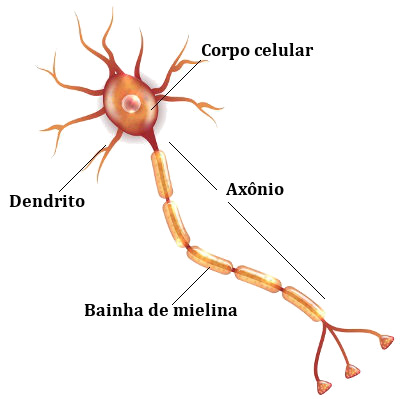
\includegraphics[height=0.3\textheight]{img/neuronio}
	\caption{Neurônio biológico e seus componentes: corpo, axônio e dendritos.}
	\label{fig:neuronio_biologico}
\end{figure}

\begin{figure}[ht]
	\centering
	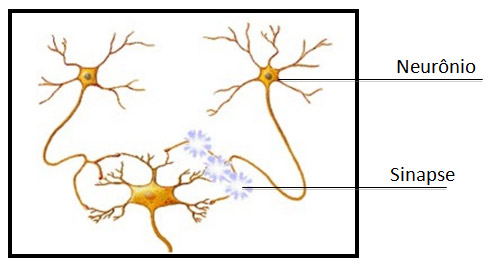
\includegraphics[width=0.6\textwidth]{img/redeneuralbiologica.jpg}
	\caption{Conexão entre neurônios biológicos}
	\label{fig:redeneuralbiologica}
\end{figure}

\begin{figure}[ht]
	\centering
	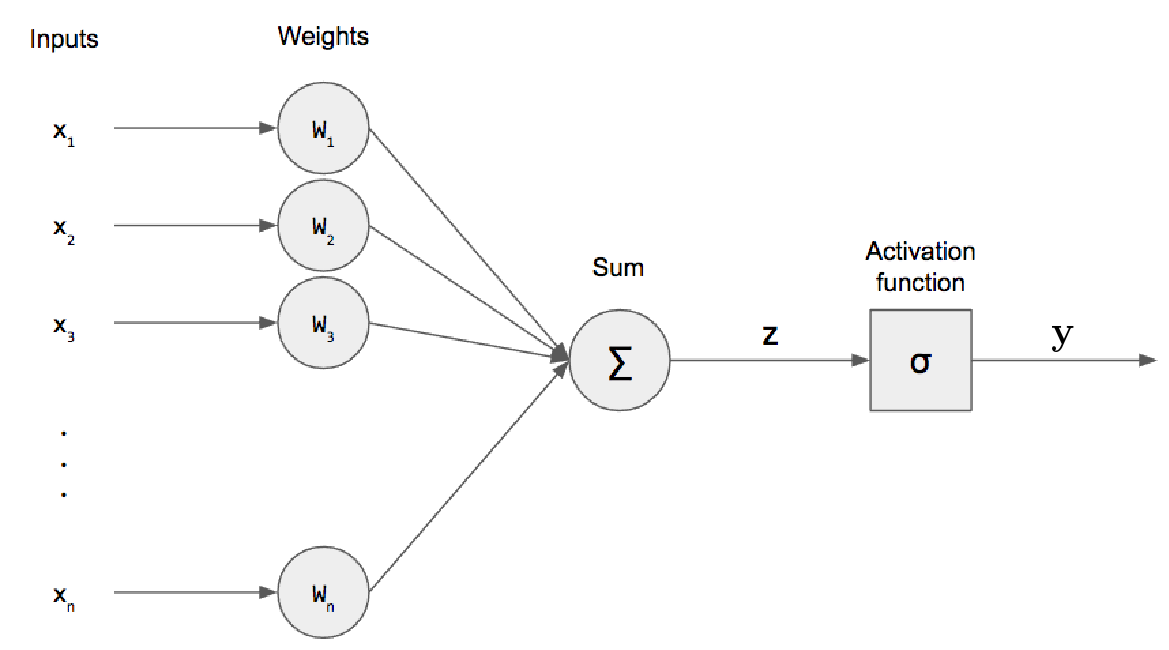
\includegraphics[width=0.7\textwidth]{img/perceptron.png}
	\caption{Neurônio Perceptron}
	\label{fig:perceptron}
\end{figure}

Com base neste modelo biológico, chegou-se ao modelo de redes neurais artificiais mais primitivo, o \emph{Perceptron}. Explanado na Figura \ref{fig:perceptron}, este modelo é formado por somente um neurônio artificial que contém $n$ terminais de entrada dada por $ x = x_1, \ldots, x_n$ e um terminal de saída $y$, uma alusão aos dendritos, centro e axônio de um neurônio biológico. A saída é mapeada através de uma função de ativação $y = g(z)$ expressa na Equação \ref{eq:funcao_neuronio}, em que a soma ponderada $z$ do vetor de entrada $x$ pelo conjunto de pesos $w = w_1, \ldots, w_n$ deve ser maior ou igual a um limiar de ativação $\theta$.

\begin{gather}\label{eq:funcao_neuronio}
	z = \sum_{i=1}^n x_i w_i\\
	y = g(z) =
		\begin{cases}
			0, & \text{se } z < \theta\\
			1, & \text{se } z \geq \theta
		\end{cases}
\end{gather}

Este modelo inicial apresentava algumas limitações devidas principalmente à sua linearidade e simplicidade, que faz com que seja possível resolver apenas problemas linearmente separáveis \cite{braga2000redes}. Um modelo Perceptron é incapaz de aprender a função XOR, por exemplo \cite{goodfellow2016deep}. Atualmente, as redes neurais artificiais possuem várias camadas de neurônios interligados, como é retratado no modelo da Figura \ref{fig:mlp}, chamado \emph{Multilayer Perceptron}. Este modelo contém uma camada de entrada, várias camadas escondidas, e uma camada de saída, e várias funções de ativação podem ser utilizadas para determinar a saída dos neurônios. Isto aumenta o escopo dos problema que podem ser resolvidos com RNAs.
\todo[inline]{-- APLICAÇÕES}

\begin{figure}[ht]
	\centering
	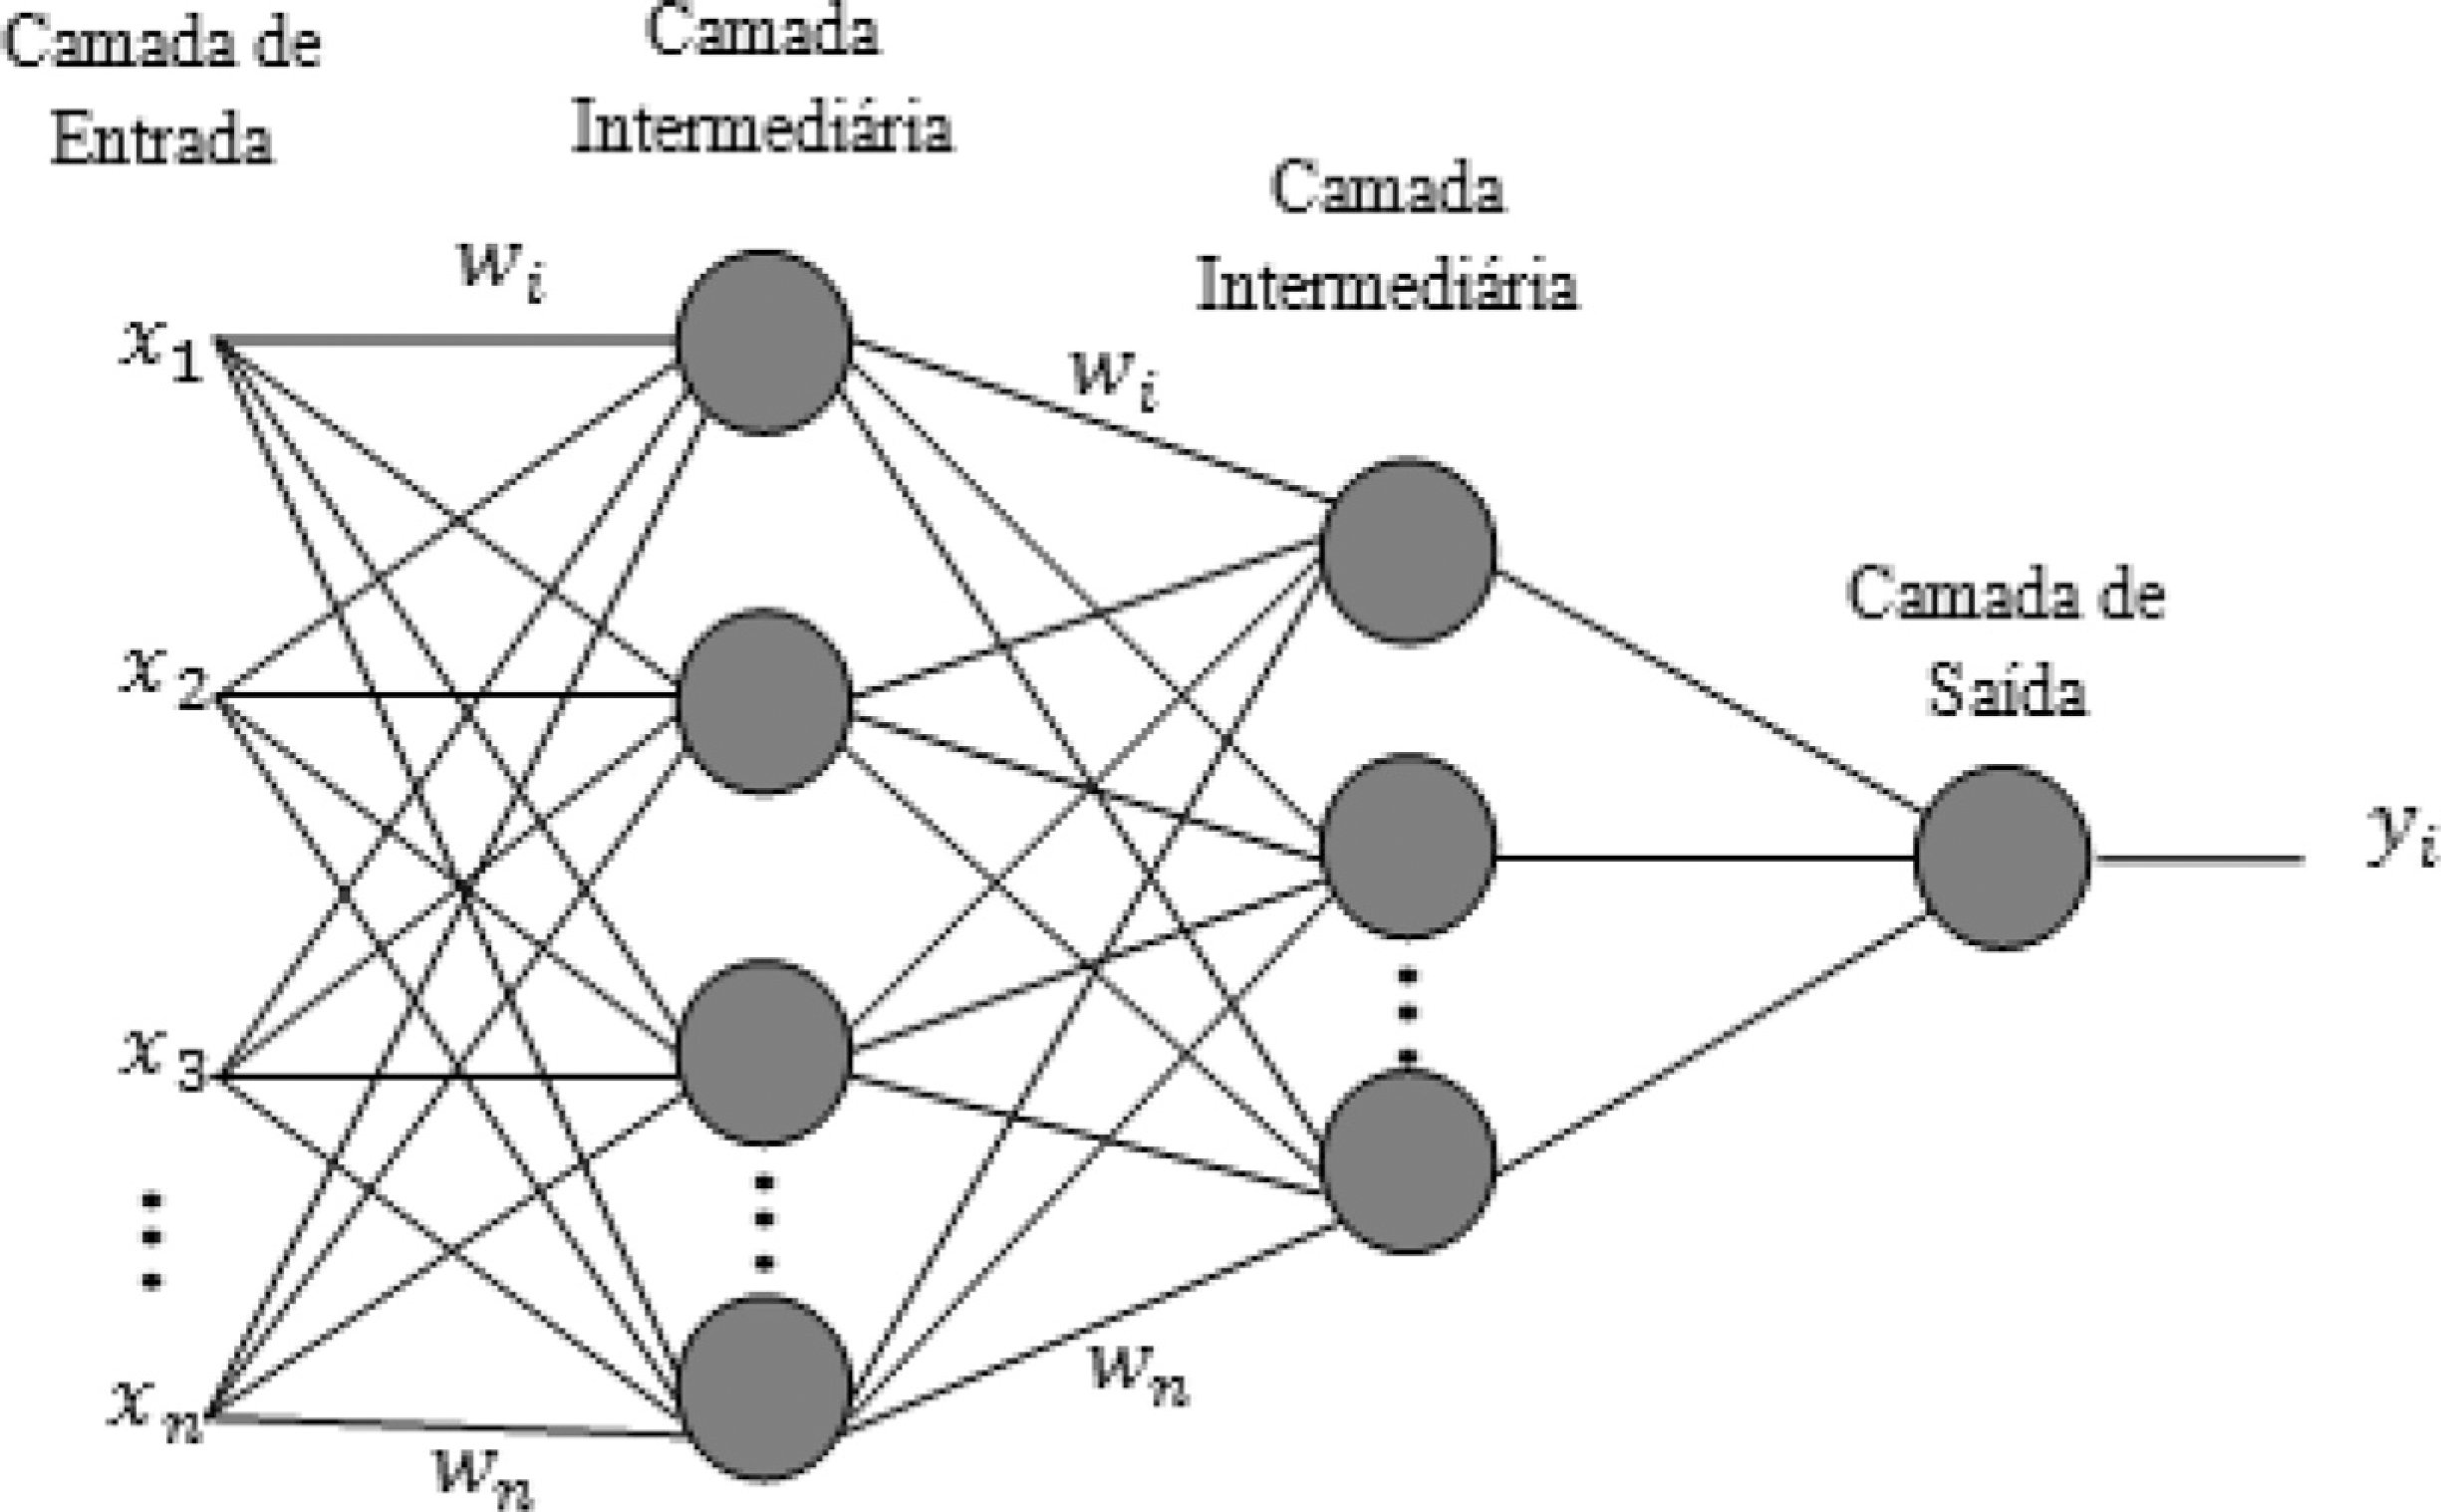
\includegraphics[width=0.7\textwidth]{img/mlprna.jpg}
	\caption{Rede Neural Multicamadas}
	\label{fig:mlp}
\end{figure}

Várias funções de ativação são utilizadas para determinar as saídas dos neurônios das camadas escondidas e de saída. As funções de ativação mais comuns são a linear ou identidade, \emph{ReLU} -- unidade exponencial linear retificada e suas variações, softmax, tangente hiperbólica e sigmoide.

\begin{table}[ht]
	\scalefont{0.8}
	\centering
	\caption{Funçoes de ativação mais populares. ---melhorar legenda}
	\label{tab:ativacoes}
	\begin{tabular}{l l p{6.5cm} l}
		\toprule
		Nome 			 		& Gráfico & Equação & Intervalo\\
		\midrule
		Identidade ou Linear		&
		 	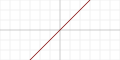
\includegraphics[width=0.1\textwidth]{img/identidade.png}
			&
			$
				\begin{aligned}
					g(z) = z
				\end{aligned}
			$
			& $(-\infty, + \infty) $\\
		\hline
		Tangente Hiperbólica		&
			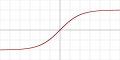
\includegraphics[width=0.1\textwidth]{img/tanh.png}
			&
			$
				\begin{aligned}
					g(z) = tanh(z) =\frac{(e^z - e^{-z})}{(e^z + e^{-z})}
				\end{aligned}
			$
			 & $(-1,1)$\\
		\hline
		Sigmoide ou Logística		&
			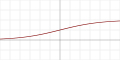
\includegraphics[width=0.1\textwidth]{img/sigmoid.png}
			&
			$
				\begin{aligned}
					g(z) = \sigma(z) = \frac{1}{1+e^{-x}}
				\end{aligned}
			$
			& $ (0,1) $\\
		\hline
		Unidade Linear Retificada	&
			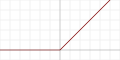
\includegraphics[width=0.1\textwidth]{img/relu.png}
			&
			$
				\begin{aligned}
					g(z) = max(0,z)
				\end{aligned}
			$
			& $ [0, \infty) $\\
		\hline
		Softmax					&
			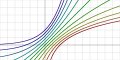
\includegraphics[width=0.1\textwidth]{img/softmax.png}
			&
			$
				\begin{aligned}
					g(\alpha, z) =
						\begin{cases}
							-\frac{ln(1-\alpha(z+\alpha))}{\alpha}, & \text{se } \alpha < 0\\
							z, & \text{se } \alpha = 0 \\
							\frac{e^{\alpha z} -1}{\alpha} + \alpha, & \text{se } \alpha > 0
						\end{cases}
				\end{aligned}
			$
			& $(-\infty, \infty)$\\
		\bottomrule
	\end{tabular}
\end{table}

\todo[inline]{redes neurais mlp; citar outros tipos de redes Neurais --MLP e Boltzmann machines}

\todo[inline]{Backpropagation --> gradiente descendente, solvers}

\todo[inline]{aplicações}
